\documentclass[11pt]{article}
\usepackage{hyperref}
\hypersetup{colorlinks=True, urlcolor=blue}
\usepackage{graphicx}
\usepackage{subfigure}
\usepackage[a4paper, total={6in, 10in}]{geometry}
\title{Khidmat -- Bird Recognition Project\\ \textit{Intermediate Progress Report}}
\author{Ali Hamza \& M. Usaid Rehman}
\date{\today}

\begin{document}

    \maketitle
    \section*{Introduction}
    \subsection*{Objective}
    Keeping track of changes in biodiversity in Pakistan is a challenge due to a lack of resources, personnel and initiatives. Therefore, tracking changes in wildlife population has become difficult which has lead to a lack of up-to-date data on biodiversity in Pakistan. 
    
    The objective of this Khidmat is to create a machine learning model that distinguishes between three different species of birds -- namely: the house sparrow, house crow, and common myna. This model will serve as the proof-of-concept for a larger model that WWF can use to identify and categorize many different species of birds.
    
    This model will fit into a larger app that would be distributed by WWF to the general public to enlist help from citizen scientists who would take pictures of birds that
    will then be identified by the model and then the data corresponding to that bird will
    be added to the WWF database. This will help remedy the issue of lack of data regarding biodiversity.
    
    \section*{Methodology}
    The following steps were initially established in order to achieve this objective:
    
    \begin{enumerate}
        \item Image Collection
        \item Image Prepossessing
        \item Feature Extraction
        \item Training
        \item Testing
        \item Results
    \end{enumerate}

    \subsection*{Image Collection}
    The images were collected from the following websites:
    \begin{enumerate}
        \item \url{https://search.macaulaylibrary.org/catalog?taxonCode=myna&mediaType=p&q=Common%20Myna}
        \item \url{https://ebird.org/media/catalog?taxonCode=commyn&mediaType=p&sort=rating_rank_desc&q=Common%20Myna%20-%20Acridotheres%20tristis}
        \item \url{https://ebird.org/media/catalog?taxonCode=houcro1&sort=rating_rank_desc&mediaType=p&regionCode=}
        \item \url{https://search.macaulaylibrary.org/catalog?taxonCode=houcro1&mediaType=p&region=Pakistan%20(PK)&regionCode=PK&q=House%20Crow%20-%20Corvus%20splendens}
        \item \url{https://www.kaggle.com/gpiosenka/100-bird-species}
        \item \url{https://search.macaulaylibrary.org/catalog?taxonCode=houspa&mediaType=p&q=House%20Sparrow}
        \item \url{https://ebird.org/media/catalog?taxonCode=houspa&mediaType=p&sort=rating_rank_desc&q=House%20Sparrow%20-%20Passer%20domesticus}
    \end{enumerate}     
    % All the images that were collected have been stored on \hyperref[]https://drive.google.com/drive/folders/18k-roE_VJSB1dcrhvN1y_EosVF7Kb0dY?usp=sharing]{Google Drive}
    All images collected: \url{https://drive.google.com/drive/folders/18k-roE_VJSB1dcrhvN1y_EosVF7Kb0dY?usp=sharing}
    \subsection*{Image Preprocessing}
    The images were preprocessed using the following steps:
    \begin{enumerate}
        \item \texttt{Find Box} Function \newline 
        Each image was taken and a Computer Vision tool was used to find a box that contains a bird-like object within it. This function would then detect all edges of the bounding-box the bird-like object has been detected to be inside. This ensure the final image only contains the bird itself.
        \item \texttt{Crop Image} Function  \newline
        Each image was then taken and cropped into a square as this would standardize each image that will be fed into the neural net. We cropped images to sizes: $50\times 50$, $100\times 100$, and $200\times 200$ as seen in \ref{Birds}
    \end{enumerate}


    \subsection*{Training $\&$ Testing}
    
    In order to build our image classification pipeline, we implemented two different 
    deep neural networks -- standard convolutional neural network, and residual network (ResNet). Convolutional neural nets (CNNs) are ideal models for image classification and are the go-to choice for most image classification tasks.
    
    Our dataset consists of 1500 images, and we have used a 70 to 30 train-test split of the data using built-in Python methods. We then trained our ResNet and CNN using the Adam optimization algorithm. The training is done using mini-batches of data chosen randomly 
    from the dataset and then optimized using gradients. 

    The results of our model has been promising. Based on our results, we determined that
    ResNet has performed better overall, giving a higher test accuracy at the end. With a CNN, our accuracy is a little over 60\%, however, with a ResNet this goes up to almost 85\% as shown in Figure \ref{lna1} and Figure \ref{lna2}.
    \section*{Remaining Work}
    
    Based on our recent discussion with Dr. Sarah Hasnain, we've decided to that the model can be made to be slightly more accurate and reach at least $90\%$ accuracy. This can be done by taking the following steps:
    \begin{enumerate}
        \item Collecting at least 50-60 more images of each bird
        \item Augmentation of the data
        \item Further fine-tuning of parameters
    \end{enumerate}
    The final model will be trained on the entire dataset and tested again. We further plan to create a detailed report at the end of this project for WWF Pakistan detailing each component of the machine learning pipe line. The report will serve as a record of the work done, and will contain documentation for the code for future developers to follow. 
    
    \vspace{5 em}
    \section*{Figures and Images}
        \begin{figure}[h!]
        \centering
        \subfigure[$50\times 50$]{
        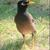
\includegraphics[]{pictures/CM1.jpg}
        }
        \subfigure[$100\times 100$]{
        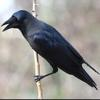
\includegraphics[]{pictures/HC4.jpg}
        }
        \subfigure[$200\times 200$ ]{
        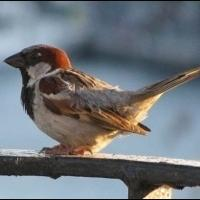
\includegraphics[]{pictures/HS2.jpg}
        }
        \caption{Preprocessed Bird Images}
        \label{Birds}
    \end{figure}
    \vspace{3 em}
    \begin{figure}[h!]
        \centering
        \subfigure{
        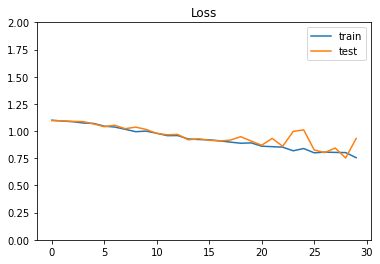
\includegraphics[scale = 0.55]{Report/pictures/loss.png}
        }
        \subfigure{
        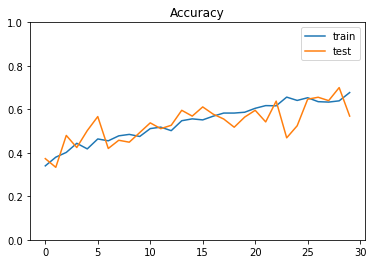
\includegraphics[scale = 0.55]{Report/pictures/accuracy.png}
        }
        \caption{Loss and Accuracy Plots with Convolutional Neural Net}
        \label{lna1}
    \end{figure}
    
    \newpage
    \begin{figure}[h!]
        \centering
        \subfigure{
        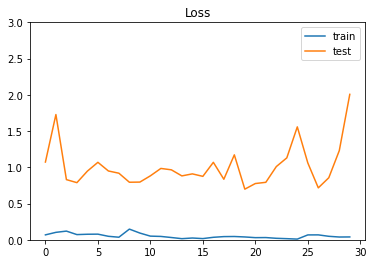
\includegraphics[scale = 0.55]{Report/pictures/loss1.png}
        }
        \subfigure{
        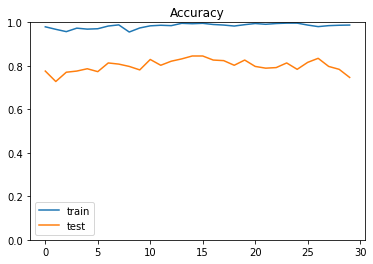
\includegraphics[scale = 0.55]{Report/pictures/accuracy1.png}
        }
        \caption{Loss and Accuracy Plots with Residual Neural Net}
        \label{lna2}
    \end{figure}
        
        
\end{document}

